%-----------------------------------------------------------------------------
%
%               Template for sigplanconf LaTeX Class
%
% Name:         sigplanconf-template.tex
%
% Purpose:      A template for sigplanconf.cls, which is a LaTeX 2e class
%               file for SIGPLAN conference proceedings.
%
% Guide:        Refer to "Author's Guide to the ACM SIGPLAN Class,"
%               sigplanconf-guide.pdf
%
% Author:       Paul C. Anagnostopoulos
%               Windfall Software
%               978 371-2316
%               paul@windfall.com
%
% Created:      15 February 2005
%
%-----------------------------------------------------------------------------


\documentclass[9pt,nocopyrightspace]{sigplanconf}

% The following \documentclass options may be useful:

% preprint      Remove this option only once the paper is in final form.
% 10pt          To set in 10-point type instead of 9-point.
% 11pt          To set in 11-point type instead of 9-point.
% authoryear    To obtain author/year citation style instead of numeric.

\usepackage{amsmath}
\usepackage{graphicx}
\graphicspath{ {./} }

\begin{document}

\special{papersize=8.5in,11in}
\setlength{\pdfpageheight}{\paperheight}
\setlength{\pdfpagewidth}{\paperwidth}

\conferenceinfo{CONF 'yy}{Month d--d, 20yy, City, ST, Country} 
\copyrightyear{20yy} 
\copyrightdata{978-1-nnnn-nnnn-n/yy/mm} 
\doi{nnnnnnn.nnnnnnn}

% Uncomment one of the following two, if you are not going for the 
% traditional copyright transfer agreement.

%\exclusivelicense                % ACM gets exclusive license to publish, 
                                  % you retain copyright

%\permissiontopublish             % ACM gets nonexclusive license to publish
                                  % (paid open-access papers, 
                                  % short abstracts)

\titlebanner{banner above paper title}        % These are ignored unless
\preprintfooter{short description of paper}   % 'preprint' option specified.

\title{Optimizing Source Code Size Using Simple Procedural Abstraction}
\subtitle{}

\authorinfo{James "Jim" Roberts}
           {UVA}
           {jpr4gc@virginia.edu}

\maketitle

\begin{abstract}
This paper explores the approach, results, and problems with one method of reducing source code and, by extension, the size of object files using procedural abstraction.
A simple algorithm is described and implemented that first searches for contiguous lists of instructions in the source code that appear in multiple locations, and then replaces each occurrence of the segment in order to shorten the overall size of the source and generated binary.
Problems with the approach used are also discussed including but not limited to the simplifying assumptions that are made that severely limit the code which can be abstracted due to instructions that must be avoided.

The results are also discussed in detail later on but to sum it up briefly; it works but not very well.
Most of the files are reduced a little, but it takes a long time to run and uses a large amount of memory, something that may not be possible on the type of system where code size would be an issue.
Several different replacement strategies are tested, and a heuristic that works fairly well is found, but there is lots of room for improvement both time and memory-wise in the construction of a suffix tree to find enumerate all segments of code that appear multiple times and the value function needed comparison of segments.

\end{abstract}

%\category{CR-number}{subcategory}{third-level}

% general terms are not compulsory anymore, 
% you may leave them out
%\terms
%remove

\keywords
procedural abstraction, suffix tree, code size, optimization

\section{Introduction}

In an age of relatively cheap memory, programmers in most cases are not burdened by the negative effects of time space tradeoffs and optimizations for space such as manual memory management and "lightweight" languages can be forgone in favor of methods that save time writing programs.

A small minority of programmers still write in languages like C where they have more control to an extent.
Fields such as embedded systems may do this, but what if simply writing in C doesn't provide a small enough memory footprint between stack, heap, globals, and code?
One option that will be explored in this paper is reducing the code size generated (in the .s and hopefully .o files) by identifying similar segments of code and pulling them into separate procedures.
If this segment of code is used in multiple locations and is small enough then by moving it into a separate location with a generated label and replacing each instance of the segment with a call to the label, the total size of the code can be reduced.
Such code will be referred to as abstractable or suitable for the remainder of this paper.

The remainder of this paper will be devoted to recording the approach, results, and problems associated with the basic approach chosen.

\section{Approach}

\begin{figure*}
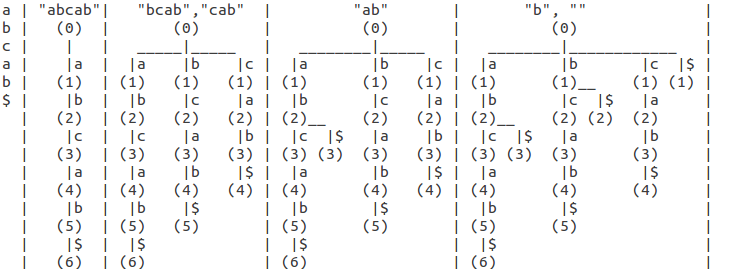
\includegraphics[width=\textwidth]{tree_diagram}
\caption{Step through the creation of a suffix tree for the string "abcab". Each node is annotated with its depth and each edge is annotated by the character mapping between the nodes. Note the implicit end of string indicator \$.}
\end{figure*}

This section will be broken down into four parts that map to the four subsections that the driver file executes.
All of the code written for this undertaking was done in Python 2.7.2 but is hopefully fairly future-proof, the creation of assembly source was done on a 32 bit machine for ease of compilation but the preprocessor should be extend-able to support 64 bit (as of now code created on a 64 bit machine will not function correctly).

The first section deals with the generation of assembly source code from a C file.
The second section deals with preprocessing a plain assembly source code file for use with the shortening algorithm.
The third section deals with creating an original copy of the code for purposes of comparing size and verifying functionality.
The final section deals with the real meat of the procedural abstraction algorithm, finding a suitable segment of code to abstract  and replacing all occurrences of it using sections from  Schaeckeler \cite{theory01} and McDowell \cite{ctci01}.

\subsection{Assembly Generation}

A filename with the .c extension will start in this stage.

GCC is called on the given source filename with the -O0 and -S flags passed creating an unoptimized assembly source file.
The driver exits if GCC returns a non-zero value.
Almost any compiler capable of creating assembly similar to GCC should be usable, GCC was chosen over the likes of Clang due to the comment free assembly, which makes comparing instructions without parsing the generated file feasible.

With the .s file generated the driver moves onto the preprocessing stage.

\subsection{Preprocessing}

A filename with the .s extension will start in this stage.

The purpose of this stage is to prepare the assembly source for the procedural abstraction function by stripping whitespace from every line, removing empty lines, removing the cfa and cfi directives which seem to be unnecessary on 32 machines and could complicate the process of replacement later on, and adding comment tags for the start and end of the "abstractable" code area as well as the previously "abstracted" code segments.

The majority of this processing is a fairly simple exercise in the use of list filters and mapping.
The only things worth noting are the strings ".text" and ".ident" which were used to locate the start and end of abstractable and abstracted code areas.

With the preprocessing complete the result is written to a file with a .orig.s extension indicating that it is the original preprocessed source.

The driver then moves on to the copy stage.

\subsection{Original Copy}

A filename with the .orig.s extension will start in this stage.

This stage simply creates a copy of the file with a .pp.s extension which is the file to be updated by the procedural abstraction function.
The existence of separate "original" and "current" files makes it easier to compare the size and functionality of the completely abstracted source.

With the .pp.s file created the driver moves on to the procedural abstraction stage.

\subsection{Procedural Abstraction}

A filename with the .pp.s extension will start in this stage.

This is the stage where the heavy lifting is done to locate a suitable segment, generate a function and replace all occurrences of the segment with a call to the generated function.
In order to achieve all this, the abstractable section of the current code will be isolated and turned into a suffix tree.
The resulting structure will then be searched to find a segment with multiple children and of suitable length.
If an abstractable segment can be found then a procedure will be generated and each occurrence of the segment will be replaced with a call to the abstracted procedure.
Each time the driver is run at most one segment will be abstracted, source can be "fully" abstracted by either running the driver on the .pp.s file until "No changes made" is indicated or passing the -f flag.

This section will start with a note on what can be successfully abstracted in this simple algorithm described by Schaeckeler\cite{theory01}.
A brief description of the suffix tree data structure used to locate viable code segments will then be provided.
Then the function used to find a good segment will be described.
Finally the replacement and actual abstract procedure creation will be touched on.

\subsubsection{What can be Abstracted}

In order to start this section a basic understanding of the C calling convention and the call/ret instructions is required.
The call instruction is an unconditional jump that pushes the return address (Program Counter + 4) onto the stack and then updates the PC to the target of the call.
The ret instruction is also an unconditional jump that gets its target by popping a word off the stack, which should be the location pushed by the corresponding call, and updating the PC to the popped word.
Because of the updates to the stack that take place during call, any instructions that use stack relative addressing or which may modify the stack (any instruction where the stack pointer is an operand) cannot be abstracted as the locations accessed would all be off by one word.

It follows from the same logic that segments with a call or ret instruction may not be abstracted because the return address could mistakenly become a parameter to the procedure call or because the wrong return address may be used if the ret instruction occurs too early in the abstracted segment.

As an extension of disallowing the call or ret instruction from being abstracted, jumps and labels are not allowed because otherwise code could jump into or out of an abstracted procedure and execute a ret instruction with the wrong return address on the stack.

In essence the only code that can be abstracted in our simple approach are basic blocks with no stack based addressing or instructions.
A list of the instructions to be avoided can be found in Appendix 1.

\subsubsection{Suffix Tree}

A suffix tree is a data structure that records all the possible suffixes (strings occurring after a segment).
It is constructed by iterating over every instruction in the abstractable code and creating an edge, representing an instruction, between the root and the node (which is created if the instruction did not already have an edge, or selected if the edge already exists).
All of the following instructions are added treating the current node as the root and starting again at the instruction after the current one.

Figure 1 illustrates this process treating single characters as instructions.

First the whole string "abcab" is added with each letter getting a new edge.
Then "bcab" and "cab" are added in the same manner.
As all three of the strings so far began with different letters, each gets its own new edge from the root.
For the next substring "ab" however, the root node already has an edge for 'a' so the existing node becomes the root and the algorithm continues.
Following this algorithm to completion will generate a complete suffix tree.
Example code can be seen in McDowell\cite{ctci01}.

To implement this functionality two classes were created SuffixTree and SuffixNode each represented by the UML diagrams in Figures 2 and 3 respectively. 

\begin{figure}
\begin{center}
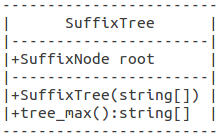
\includegraphics{tree}
\caption{High level overview of SuffixTree class.}
\end{center}
\end{figure}

\begin{figure}
\begin{center}
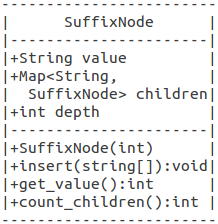
\includegraphics{node}
\caption{High level overview of SuffixNode class.}
\end{center}
\end{figure}

The SuffixTree constructor behaves similarly to the one described by \cite{ctci01}, creating an empty root node, and iterating over every sublist(i) for i from 0 to the length of the list, calling insert on root with the sublist. 

The SuffixNode constructor is also fairly basic taking the depth of the node and initializing the children map.
SuffixNode insert takes the remaining list of instructions, stores the head as the value of the node, then finds the child node to insert the rest of the code list in.
The child node will be found in the children mapping or, if there is not an existing node then, a new SuffixNode will be created with (depth+1) and added to the children mapping.
The SuffixNode count\_children method recursively finds the number of "branches" made after this node, this provides a rough estimate of the number of times this segment could be replaced in the code, which can be used as part of metric to compare nodes.

Once the suffix tree has been constructed, the duplicated segments of code can be found.

\subsubsection{Find Segment}

\begin{table*}
\begin{center}
\begin{tabular}{|l|r|r|r|r|r|r|r|r|} \hline
&lines .s&bytes .o&lines .s&bytes .o&lines .s&bytes .o&lines .s&bytes .o\\ \hline
clock.orig.s&354&5343&354&5343&354&5343&354&5343\\ \hline
clock.pp.s&352&5285&352&5261&351&5226&352&5261\\ \hline
double.orig.s&51&694&51&694&51&694&51&694\\ \hline
double.pp.s&51&694&51&694&51&694&51&694\\ \hline
fcyc.orig.s&507&8053&507&8053&507&8053&507&8053\\ \hline
fcyc.pp.s&496&7732&495&7653&494&7627&495&7653\\ \hline
Fibonacci.orig.s&448&7619&448&7619&448&7619&448&7619\\ \hline
Fibonacci.pp.s&442&7469&441&7388&440&7320&442&7442\\ \hline
play.orig.s&254&3530&254&3530&254&3530&254&3530\\ \hline
play.pp.s&254&3530&254&3530&254&3506&254&3530\\ \hline
replicated.orig.s&75&1069&75&1069&75&1069&75&1069\\ \hline
replicated.pp.s&75&1069&70&947&70&947&70&947\\ \hline
rosetta.orig.s&867&13565&867&13565&867&13565&867&13565\\ \hline
rosetta.pp.s&850&13119&849&12979&848&12960&849&12979\\ \hline
&&&&&&&&\\ \hline
Max reduction&17&446&18&586&19&605&18&586\\ \hline
Total reduction&36&975&44&1421&48&1593&43&1367\\ \hline
Mean reduction&5.142&139.285&6.285&203.000&6.857&227.571&6.142&195.285\\ \hline
Mean \% reduction&1.408&2.445&1.721&3.563&1.877&3.995&1.682&3.428\\ \hline
&&&&&&&&\\ \hline
Value Function&line estimate&&$d^{1} c^{1}$&&$d^{2} c^{1}$&&$d^{1} c^{2}$&\\ \hline
\end{tabular}
\caption{Resulting line counts and size in bytes of the original and abstracted files. The files were run through the driver until no segments of code could be abstracted (using the -f flag). Note that the absence of a decrease in line count does not mean that no procedures were abstracted or that the generated object file was not smaller.}
\end{center}
\end{table*}


Inevitably some instructions will be repeated throughout the code, ret or push \%ebp for example.
The goal of procedural abstraction though is to find repeated segments that are longer and/or appear more frequently in the source.
This insight will tailor the way that a segment is deemed to be suitable.
This manifests itself in the SuffixNode get\_value() method.

The get\_value() method provides a way to compare nodes which is necessary to find a single segment to abstract each time the driver is run.
A value function of the form $V(c,d)$ is used where $c$ is the number of children this node will have and $d$ is the depth of the node(which is equivalent the number of instructions that will be replaced).
Tweaking the value function causes the program to pick different segments to abstract.
Below are two general functions which were tried.

The first function used is:
\begin{center}
$V(c,d)=c*(d-1)-(d+2)$
\end{center}
This function estimates the number of lines that will be saved by abstracting this segment.
The logic is that $\Delta lines=numReplacements*\Delta codeRemoved - sizeOfProcedure$.
In other words by calculating the amount of code removed ($d-1$ keeping in mind that each segment is replaced with 1 call instruction) by each location where the segment occurs ($*c$) and subtracting the extra space required to replicate the segment in the abstracted section of code ($d+2$ for the extra label and ret instruction required) the net change in lines can be calculated.
Note that this is only an estimate whose flaw can be demonstrated with a trivial example of replacing "aa" in the string "aaa" where it may appear to the program as it is traversing that it can be done twice due to the number of children created, but in reality the replacement can only be done once

The second suggestion for calculating a value for the node is the formula:
\begin{center}
$V(c,d)=c^{x}d^{y}$
\end{center}
This function is designed to select segments that either appear more frequently in the code or those which are longer.
The variables $x$ and $y$ can be changed in order to weight the number of replacements ($x$) or the number of instructions replaced ($y$) more heavily.
The effects of changing the constants one can be seen in Figure 4.

\begin{figure}
\begin{center}
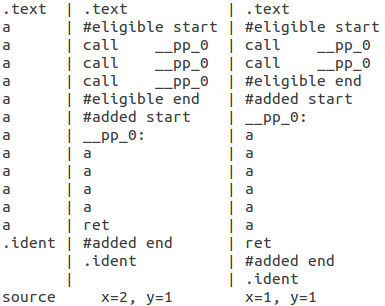
\includegraphics[scale=.8]{weightex}
\caption{The effects of weighting the number of replacements more heavily.}
\end{center}
\end{figure}

With a completed value method the SuffixTree tree\_max method can be implemented.
The actual tree\_max method is just a wrapper that tracks the best code segment found so far and its value, and calls a recursive search function on the root node.

The search function is a recursive function that accesses every node in the SuffixTree and gets its value, it takes a node and the code list so far as parameters.
Each time the search function is called on a non empty node first the length of the code is compared to 2 and the value of the node is compared to the best value so far.
If the number of instructions is greater than or equal to 2 and the value of the current node is greater than the best value so far then a copy of the code is stored and the best value is updated.

After the optional update stage all of the keys in the current node's children map are iterated over and the search code is called again on the values for each key with the current instruction appended to the list of instructions.
There is another important condition that is checked before calling the search function on each value which is that the value must not contain any of the instructions/symbols which would alter/rely on the stack or cause the segment not to be a basic block.
Without this restriction a segment may be selected which should be un-abstractable.

When the traversal has finished a single segment remains and is used as the basis for the replacement procedure.
If no segment is found then the original program is returned and the driver will terminate.

Observant readers may wonder why a value of 2 is specified.
This number is derived from the way that a code segment is abstracted where each occurrence of a segment is replaced by a call instruction, and the segment is surrounded by a label and a ret instruction.
If segments of length 1 were replaced then no matter how many occurrences of the instruction there were, the size of the code would increase because of the 3 line overhead.
If segments of length 2 are replaced then each replacement reduces the code size by 1 so 4 replacements are required to break even.
Without loss of generality segments longer than 2 instructions can also be replaced with enough matches.

\subsection{Procedure Generation}

With an abstractable segment identified the abstract procedure must be generated.
This procedure requires 3 parts, a prologue, the code segment, and an epilogue.

The prologue is simply a unique label, it can be generated by taking a prefix and appending to it a number and a colon.
The number to append can be found by counting all occurrences of colons (indicating labels) in the previously abstracted portion of the program and adding 1.
Because all of the abstracted procedures are basic blocks no other colons will be present in the code.

The code segment is the one found previously.

The epilogue is simply a ret instruction as that will return control to the location where the abstracted procedure was called.

With the procedure generated the segment can then be replaced.

\subsubsection{Segment Replacement}

With a suitable segment found the program shifts to replacing all occurrences of the segment in the abstractable code list that it possibly can.

A simple loop is used iterating over each index in the abstractable code list stopping when there are more instructions in the segment then are remaining in the abstractable code list.
At each iteration in this loop the next instructions are compared to the segment and if the next $d$ instructions match, where $d$ is the length of the segment being replaced, then the $d$ instructions are replaced with a single call to the temporary function whose label has been calculated already.

Once this loop has terminated the abstractable code will have had all occurrences of the segment removed and replaced with a call to the abstracted procedure.

The driver can then write the new .pp.s file to disk.

\section{Results}

The algorithm successfully shortens code, although not necessarily by large amounts.

Some example results are shown above in Table 1 for seven files abstracted to completion.
As shown the largest decrease in absolute size was by about 19 lines/605 bytes and the largest relative decrease in size in 6.66\% in lines/11.41\% in bytes for a file designed to perform replicated operations.
One out of the seven files had no reduction in size at all, and three out of the six files with a reduction were reduced by less than 10 lines.

Files abstracted using the $d^{2}c^{1}$ value function yielded the best results across the board in terms of both line count and object file size with an average line reduction of 6 and an average byte reduction of 227.
It also had an interesting result of reducing the object file size while maintaining the same line count in the play.c source.
This highlights another problem with the value functions where only line counts were considered and not the actual size of instructions.
As a general rule though it would seem like value functions which weigh the length of the code segment being replaced over the number of replacements being made are about 10\% more successful in reducing the size in bytes and number of lines for the inputs tested.
In addition, it appears that the line estimating function would need to be tweaked to find the actual number of replacements that can be made ahead of time, or consider the difference in bytes and not lines, or both, in order to be effective.

While the algorithm was successful in the sense that it does what it was designed to do for a majority of the files, its usefulness is limited by the small decreases in code size that it is able to obtain.
Combined with the relatively large footprint of the abstracting program itself then, it would not appear to be a particularly good solution in its current form.

Interestingly, code generated on a 64 bit machine was reduced more than on the 32 bit machine which the testing was done on.
A brief comparison of the difference between both sources revealed that the 64 bit compiler generated more frame relative instructions.
However as the code did not retain its functionality, more work would be required to determine if this strategy makes more sense on a different architecture.

\section{Problems and Improvements}

At this point a reader might be wondering where everything went wrong, the algorithm seems so simple, everything makes sense, etc. but it turns out that some fairly crippling assumptions were made along the way in order to achieve simplicity.

The first and probably most limiting assumption made was the list of instructions and symbols that could not be abstracted.
As mentioned earlier this limitation was imposed in order to ensure that all abstracted functions were essentially basic blocks with no instructions that used the stack pointer.
While these limitations allowed us to have a low overhead of two lines of code per segment and one line of code per replacement, as well as making segment selection simpler, it severely hindered our ability to find long suitable code segments due to the rampant use of stack relative addressing and calls within most 32 bit C code generated.
One possible way to circumvent this would be to change the calling convention around the abstracted code by maintaining a stack of return addresses for the temporary functions and simply popping one off and placing it on the stack before every ret inside of an abstracted function.
The biggest downside to this apart from the relative complexity that it adds is a sizable number of instructions that must be added to the code in order for it to function.

The second issue with the code as written is with the time and memory usage.
Due to the use of recursion in creating the tree and the lack of tail-recursion optimization in interpreted Python, files with an abstractable code size larger than the maximum recursive depth allowed by python will never be improved.
While converting the recursive creation of the tree could be done fairly easily without additional memory or time, in order for anything to change the function that searches for the segment to replace would also need to be converted to iterative form.
Seeing as the search function is not simply tail recursive, as it is essentially performing a depth first search, a rather large stack would be required to hold many nodes, and the order $O(n)$ list operations would still be a problem.
Running time is also an issue due to the tree creation being $O(n^{2})$, assuming that list operations such as slicing takes constant time, in the number of abstractable lines alone.
Tacking on a few more tree traversals and many list slicing/concatenation operations causes the program to run fairly slowly.
The solution to both of these issues would appear to be using additional data structures to hold information in a quickly accessible fashion that doesn't impact the recursive depth.
Unfortunately this would not only drive the memory footprint up which would be concerning in a program designed to cut down the memory usage of programs.

Another problem encountered was the naivete of the value function used to aid the selection of an abstractable segment.
It had two main problems, first it considered each line to be an equal size both for the number of instructions and the size in bytes of said instructions.
With a little more information from the compiler, including the addressing mode used for each call, it should be possible to generate a mapping from instruction to size in bytes for a more accurate number.
The second problem is that knowing the exact number of replacements that could be made for a specific segment is difficult without pretending to replace the segment as part of the value calculation.
The other option is to try and compute the number of places ahead of time by maintaining a list of which locations in the code are associated with each node and discounting any locations that are closer together than the length of the segment.
Unfortunately either solution would mean an even larger time or memory footprint on an already slow and relatively large program.
Instead we settle on a weighted approximation that provides the best results.

\section{Conclusion}

In this paper we set out to answer a seemingly simple question: "What can I do if I've written code that has as small of a source size as I possibly can write but it needs to be smaller?" by using procedural abstraction.
The basic algorithm laid out can reduce the size of code by finding repeated segments of code which could be replaced with a call to a single procedure containing the code.
While at first glance it may have seemed like an easy problem in the same vein as finding common substrings it turned out to be fairly difficult to do well programmatically.

We have stepped through the process of generating assembly source code, preprocessing it, as well as finding a suitable segment of code to abstract using a SuffixTree and actually replacing it.
This has also included some discussion of the problems and challenges associated with finding a good piece of code to replace and how the simplifying assumptions that you make can limit the effectiveness of the algorithm.

While all of the information required to replicate this project or create a similar one has hopefully been provided, a glance at the results should serve as a warning against attempting this basic approach unless it is simply an exercise or you are willing to dig deeper on your own and fix some of the problems that were pointed out.
All in all when considering the question posed, it would seem like a better approach to try at first would be to simply use the -Os flag for GCC or your favorite compiler.

\appendix
\section{Appendix}

\subsection{Instructions/Symbols to Avoid Abstracting}
":", "jo", "js", "je", "jz", "jb", "jc", "ja", "jl", "jg", "jp", "jno", "jne", "jnz", "jnb", "jae", "jnc", "jbe", "jna", "jge", "jnl", "jle", "jng", "jpe", "jnp", "jpo", "pop", "ret", "esp", "rsp", "jnae", "jnbe", "jnge", "jnle", "jcxz", "call", "push", "jecxz"
\\ List of jump instructions from \cite{intel01}

\acks

I would like to thank Professors Weimer and Tychonievich for several discussions that helped me to establish a viable idea for this project, as well as some suggestions for ways to approach the problem.

% We recommend abbrvnat bibliography style.

\bibliographystyle{abbrvnat}

% The bibliography should be embedded for final submission.

\begin{thebibliography}{}
\softraggedright

\bibitem[Schaeckeler et~al.(2009)]{theory01}
Stefan Schaeckeler and Weijia Shang. 2009. Procedural Abstraction with Reverse Prefix Trees. In Proceedings of the 7th annual IEEE/ACM International Symposium on Code Generation and Optimization (CGO '09). IEEE Computer Society, Washington, DC, USA, 243-253. DOI=10.1109/CGO.2009.25 http://dx.doi.org/10.1109/CGO.2009.25

\bibitem[McDowell (2013)]{ctci01}
Gayle Laakmann McDowell. 2013. Cracking the Coding Interview 5th ed. CareerCup , LLC, Palo Alto, CA, USA

\bibitem[Intel (2014)]{intel01}
Intel. 2014. Intel 64 and IA-32 Architectures Software Developer's Manual Colume 2(2A, 2B, \& 2C): Instruction set Reference, A-Z. Intel, Santa Clara, CA, USA http://www.intel.com/content/dam/www/public/us/en/documents/manuals/64-ia-32-architectures-software-developer-instruction-set-reference-manual-325383.pdf

\end{thebibliography}


\end{document}

%                       Revision History
%                       -------- -------
%  Date         Person  Ver.    Change
%  ----         ------  ----    ------

%  2013.06.29   TU      0.1--4  comments on permission/copyright notices

